\documentclass[11pt,a4paper]{article}
\usepackage[T1]{fontenc}
\usepackage[utf8]{inputenc}
\usepackage{lmodern}
\usepackage[margin=2.3cm]{geometry}
\usepackage{graphicx}
\graphicspath{{../img/}}
\usepackage{xcolor}
\definecolor{spblue}{HTML}{1F4E79}
\definecolor{spteal}{HTML}{2C7A7B}
\usepackage{booktabs}
\usepackage{longtable}
\usepackage{array}
\usepackage{enumitem}
\usepackage{float}
\usepackage{caption}
\captionsetup{font=small,labelfont=bf}
\usepackage{listings}
\lstset{basicstyle=\ttfamily\footnotesize,breaklines=true,frame=single,backgroundcolor=\color{gray!8},columns=fullflexible,keepspaces=true}
\usepackage[hidelinks]{hyperref}
\usepackage{titlesec}
\titleformat{\section}{\color{spblue}\Large\bfseries}{\thesection}{0.6em}{}
\titleformat{\subsection}{\color{spteal}\large\bfseries}{\thesubsection}{0.6em}{}
\setlength{\parskip}{0.5em}\setlength{\parindent}{0pt}

\title{ScholarPath --- From EERD to Relational Schema\\[0.3em]\large Step 3: Relational Mapping}
\author{ScholarPath Team}
\date{}

\begin{document}
\maketitle

\begin{abstract}
\noindent This is Part~3 of a four-part teaching series that walks the ScholarPath
data model from a plain Entity--Relationship Diagram (ERD) through an Enhanced
ER Diagram (EERD), then into a \emph{relational schema}, and finally into
object-oriented Class Diagrams. Here we take the EERD produced in Part~2 and
convert it into concrete relations (tables, keys, and foreign keys) by applying
Elmasri \& Navathe's classic seven/nine-step ER/EER-to-relational mapping
algorithm. Every rule is illustrated with a real ScholarPath construct, and
every claim is reconciled against the \emph{live} Azure SQL schema (the deployed
EF~Core model snapshot), so the mapping you see is the schema that actually
runs in production --- 62 tables in total. Where ScholarPath deliberately
deviates from the textbook (multivalued attributes stored as JSON, a
single-table specialization, loose references on high-volume tables), the
deviation is stated plainly rather than hidden. The companion documents are
\emph{ScholarPath --- ERD} (Part~1), \emph{ScholarPath --- EERD} (Part~2), and
\emph{ScholarPath --- Class Diagrams} (Part~4).
\end{abstract}

\tableofcontents

\section{Goal: turning the EERD into relations}

The EERD from Part~2 is a \emph{conceptual} model: it speaks of entities,
relationships, cardinalities, weak entities, and specialization. A relational
database, by contrast, knows only \emph{relations} (tables), \emph{attributes}
(columns), \emph{primary keys}, and \emph{foreign keys}. Step~3 is the
disciplined translation between the two worlds.

We follow the standard algorithm presented by Elmasri \& Navathe
(\emph{Fundamentals of Database Systems}), commonly stated in seven core steps
(plus two for the EER extensions of specialization and union), giving the
``seven/nine-step'' mapping. The algorithm is attractive for a defense because
it is \emph{mechanical and auditable}: each conceptual construct has exactly one
prescribed rule, so a reviewer can trace any table in the schema back to the
EERD element that produced it.

Two ground rules shaped our application of the algorithm:

\begin{itemize}[leftmargin=1.4em]
  \item \textbf{Fidelity to the deployed schema.} The result was reconciled
        against the live EF~Core model snapshot
        (\texttt{ApplicationDbContextModelSnapshot.cs}) and the production Azure
        SQL dump. Where the textbook ideal and the shipped schema differ, we
        document the \emph{shipped} schema and flag the deviation.
  \item \textbf{Honesty about denormalization.} A graduation project that
        claims perfect third-normal-form purity invites a hard question at
        defense. Instead we record the pragmatic choices (JSON multivalued
        columns, single-table inheritance, loose references) and justify each.
\end{itemize}

A short notation reminder, used throughout this document and in the figures:

\begin{itemize}[leftmargin=1.4em]
  \item \underline{Underlined} attribute = primary key. All primary keys are
        \texttt{Guid} (\texttt{uniqueidentifier}) unless noted; junction tables
        use a \emph{composite} primary key.
  \item \emph{Italic} attribute = foreign key, with its delete rule
        (\textbf{Cascade}, \textbf{Restrict}, or \textbf{SetNull}).
  \item \textbf{(soft)} marks a \emph{loose reference}: a \texttt{Guid} that
        points at another relation logically but carries \emph{no}
        \texttt{FOREIGN KEY} constraint --- integrity is enforced in
        application code. This is a deliberate decoupling for
        high-volume / audit / analytics relations.
  \item \texttt{$\star$UK} = unique index/constraint;
        \texttt{FUK} = \emph{filtered} (partial) unique index;
        \texttt{enc} = encrypted column; \texttt{cents} = money stored as
        integer cents.
  \item \texttt{\{audit\}} abbreviates the auditing columns
        (\texttt{CreatedAt}, \texttt{CreatedByUserId}, \texttt{UpdatedAt},
        \texttt{UpdatedByUserId}, \texttt{RowVersion}); \texttt{\{softdel\}}
        abbreviates the soft-delete columns
        (\texttt{IsDeleted}, \texttt{DeletedAt}, \texttt{DeletedByUserId}).
\end{itemize}

\section{The mapping algorithm at a glance}

Table~\ref{tab:algo} restates Elmasri \& Navathe's nine steps and, for each,
names the place(s) in ScholarPath where that construct actually appears. The
rest of the document then walks the constructs one by one.

\begin{table}[H]\centering
\caption{The ER/EER-to-relational mapping algorithm, applied to ScholarPath.}
\label{tab:algo}
\small
\begin{longtable}{@{}c>{\raggedright\arraybackslash}p{2.7cm}>{\raggedright\arraybackslash}p{4.6cm}>{\raggedright\arraybackslash}p{5.2cm}@{}}
\toprule
\textbf{Step} & \textbf{Construct} & \textbf{Rule applied} & \textbf{Where it appears in ScholarPath} \\
\midrule
\endhead
1 & Regular (strong) entity & One relation; choose a primary key. &
\texttt{Users}, \texttt{Scholarships}, \texttt{Bookings}, \dots\ (every strong entity). \\
\addlinespace
2 & Weak entity & Relation including the owner's PK as part of an identifying FK;
identity = owner PK + partial key. &
\texttt{Scholarship\_Children}, \texttt{Application\_Children},
\texttt{Education\_Entries}, \texttt{Resource\_Chapters},
\texttt{*\_Files/\_Links}. \\
\addlinespace
3 & 1:1 relationship & FK (plus \texttt{$\star$UK}) on the side with total
participation. &
\texttt{Users}--\texttt{UserProfiles}; \texttt{Bookings}--\texttt{ConsultantReviews};
\texttt{Applications}--\texttt{CompanyReviews};
\texttt{AiInteractions}--\texttt{AiRedactionAuditSamples};
\texttt{Users}--\texttt{UserRiskFlags}. \\
\addlinespace
4 & 1:N relationship & FK on the N-side referencing the 1-side. &
\texttt{Scholarships}$\rightarrow$\texttt{Applications},
\texttt{Users}$\rightarrow$\texttt{Bookings},
\texttt{ForumPosts}$\rightarrow$\texttt{ForumVotes}, \dots \\
\addlinespace
5 & M:N relationship & New relationship relation with composite PK = the two
FKs. &
\texttt{UserRoles} (User\,$\bowtie$\,Role),
\texttt{ForumPostTags} (Post\,$\bowtie$\,Tag);
\texttt{SavedScholarships} is the same shape but uniqueness-only (loose). \\
\addlinespace
6 & Multivalued attribute & Separate relation keyed by (owner PK + value). &
Realized as JSON columns (\texttt{PreferredCountriesJson}, \texttt{TagsJson},
\dots) \emph{or} child rows (\texttt{Scholarship\_Children}) --- see the
deviation note. \\
\addlinespace
7 & N-ary relationship & New relation with a FK to each participant. &
\texttt{CompanyReviewRequests} (Student $\times$ Company $\times$ Scholarship
$\times$ Payment). \\
\addlinespace
8 & Specialization / generalization (EER) & \emph{Option~C} --- single relation
with a type discriminator. &
User \textbf{ISA} \{Student, Company, Consultant, Admin\}: one \texttt{Users}
table + role rows in \texttt{UserRoles}; role-specific columns folded into one
\texttt{UserProfiles} relation (NULL when not applicable). \\
\addlinespace
9 & Union / category (EER) & --- &
Not used (no category/union types in the model). \\
\bottomrule
\end{longtable}
\end{table}

\section{Walking each construct with ScholarPath examples}

\subsection{Step 1 --- Strong (regular) entities}

Each strong entity becomes exactly one relation, and we pick its primary key.
ScholarPath uses surrogate \texttt{Guid} keys throughout (rather than natural
keys), which keeps foreign keys uniform and avoids leaking business meaning into
identifiers. \texttt{Users}, \texttt{Scholarships}, \texttt{Bookings},
\texttt{Resources}, \texttt{ForumPosts}, \texttt{Payments}, and the lookup
tables (\texttt{Categories}, \texttt{Roles}, \texttt{ForumTags},
\texttt{ExpertiseTags}) are all step-1 relations.

The principal example is the \texttt{Users} relation, which carries the
ASP.NET~Identity attributes:

\begin{lstlisting}[language=SQL]
USERS( Id, Email, NormalizedEmail, FirstName, LastName, PasswordHash,
       SecurityStamp, ConcurrencyStamp, EmailConfirmed, PhoneNumber,
       LockoutEnd, LockoutEnabled, AccessFailedCount, TwoFactorEnabled,
       ProfileImageUrl, AccountStatus, ActiveRole, IsOnboardingComplete,
       PreferredLanguage, CountryOfResidence, LastLoginAt, {audit}, {softdel} )
\end{lstlisting}

A subtle, defense-relevant point: e-mail uniqueness here is \emph{not} a
database unique constraint. Identity creates a unique filtered index on
\texttt{NormalizedUserName} but a \emph{non-unique} index on
\texttt{NormalizedEmail}; e-mail uniqueness is enforced by the Identity
validator in application code. This is the first of several places where
``what the model promises'' and ``what the database enforces'' diverge --- a
theme we return to in Section~\ref{sec:accuracy}.

\subsection{Step 2 --- Weak entities and identifying cascades}

A weak entity has no key of its own; it is identified only \emph{relative to its
owner}. The rule produces a relation that embeds the owner's primary key as part
of an identifying foreign key, and --- crucially --- that foreign key cascades
on delete, because a weak-entity row is meaningless once its owner is gone.

ScholarPath's clearest weak entities are the \texttt{*\_Children} and
\texttt{Education} rows:

\begin{lstlisting}[language=SQL]
EDUCATION_ENTRIES( Id, UserProfileId, InstitutionName, Degree, FieldOfStudy,
       StartDate, EndDate, Gpa(4,2), Description, {audit} )
    FK UserProfileId -> USER_PROFILES(Id)  [Cascade]      -- identifying owner

SCHOLARSHIP_CHILDREN( Id, ScholarshipId, ChildType, KeyEn, KeyAr,
       ValueEn, ValueAr, SortOrder )
    FK ScholarshipId -> SCHOLARSHIPS(Id)  [Cascade]       -- weak EAV entity

APPLICATION_CHILDREN( Id, ApplicationTrackerId, ChildType, Title, Content,
       MetadataJson, OccurredAt, ActorUserId(soft), SortOrder )
    FK ApplicationTrackerId -> APPLICATIONS(Id)  [Cascade] -- status history / notes
\end{lstlisting}

Note that \texttt{Education\_Entries} hangs off \texttt{UserProfiles}, not
directly off \texttt{Users} --- educational history is owned by the profile.
The \texttt{Scholarship\_Children} and \texttt{Application\_Children} relations
are entity--attribute--value (EAV) carriers: a single weak relation holds many
heterogeneous child rows discriminated by a \texttt{ChildType} column (e.g.\ a
scholarship's benefits and eligibility bullets, or an application tracker's
status-history and note events). The same step-2 pattern produces
\texttt{Resource\_Chapters} (owned by \texttt{Resources}) and the
\texttt{UpgradeRequest\_Files}/\texttt{UpgradeRequest\_Links} relations (owned by
\texttt{UpgradeRequests}). In every case the identifying FK is
\textbf{Cascade}, faithfully realizing the existence-dependency of the EERD.

\subsection{Step 3 --- 1:1 relationships}

For a one-to-one relationship the algorithm places the foreign key on the side
with \emph{total} participation and backs it with a unique constraint so the
``one'' is enforced. ScholarPath has five textbook 1:1 relationships:

\begin{itemize}[leftmargin=1.4em]
  \item \texttt{Users}--\texttt{UserProfiles}: every profile belongs to exactly
        one user; the FK \texttt{UserId} carries a \texttt{$\star$UK}.
  \item \texttt{Bookings}--\texttt{ConsultantReviews}: at most one review per
        completed booking.
  \item \texttt{Applications}--\texttt{CompanyReviews}: at most one company
        review per application.
  \item \texttt{AiInteractions}--\texttt{AiRedactionAuditSamples}: at most one
        privacy-audit sample per AI interaction.
  \item \texttt{Users}--\texttt{UserRiskFlags}: at most one churn-risk flag row
        per user.
\end{itemize}

\begin{lstlisting}[language=SQL]
USER_PROFILES( Id, UserId*UK, Biography enc, ..., {audit} )
    FK UserId -> USERS(Id)  [Restrict]      -- 1:1, *UK enforces "exactly one"

CONSULTANT_REVIEWS( Id, BookingId*UK, StudentId, ConsultantId, Rating, ... )
    FK BookingId -> BOOKINGS(Id)  [Restrict]  -- *UK => one review per booking
\end{lstlisting}

The unique index on the FK is what upgrades a plain 1:N foreign key into a 1:1
relationship at the database level. (All of these FKs into \texttt{Users} use
\textbf{Restrict}, for reasons explained in Section~\ref{sec:refint}.)

\subsection{Step 4 --- 1:N relationships}

The most common construct: place the foreign key on the ``many'' side,
referencing the ``one'' side. Examples are everywhere ---
\texttt{Scholarships}$\rightarrow$\texttt{Applications},
\texttt{Users}$\rightarrow$\texttt{Bookings},
\texttt{ForumPosts}$\rightarrow$\texttt{ForumVotes},
\texttt{Resources}$\rightarrow$\texttt{ResourceChapters}, and the self-reference
\texttt{ForumPosts}$\rightarrow$\texttt{ForumPosts} (a reply points to its parent
post; a \texttt{NULL} parent marks a root thread). Many of these FKs are paired
with composite indexes (e.g.\ \texttt{(Status, Deadline)} on
\texttt{Scholarships}) to support the common query paths.

\subsection{Step 5 --- M:N relationships (junction relations)}

A many-to-many relationship cannot be represented by a single foreign key, so
the algorithm introduces a new \emph{relationship relation} (junction table)
whose primary key is the composite of the two foreign keys. ScholarPath has two
true junction tables:

\begin{lstlisting}[language=SQL]
USER_ROLES( UserId, RoleId )                 -- M:N junction (User <-> Role)
    FK UserId -> USERS(Id)  [Restrict]       -- NO ACTION: no FK cascades from Users
    FK RoleId -> ROLES(Id)  [Cascade]
    PK = (UserId, RoleId)

FORUM_POST_TAGS( ForumPostId, ForumTagId )   -- M:N junction (Post <-> Tag)
    FK ForumPostId -> FORUM_POSTS(Id)  [Cascade]
    FK ForumTagId  -> FORUM_TAGS(Id)   [Cascade]
    PK = (ForumPostId, ForumTagId)
\end{lstlisting}

A near-miss worth pointing out is \texttt{SavedScholarships} (a student's
bookmarked scholarships). It is conceptually an M:N association, and it uses the
same shape, \emph{but} it is realized with \textbf{uniqueness only}: it has its
own surrogate \texttt{Id}, a real FK to \texttt{Scholarships}, and a unique index
on \texttt{(UserId, ScholarshipId)} --- while the \texttt{UserId} leg is a
\emph{loose} reference (no FK). This keeps the bookmark table decoupled from the
\texttt{Users} principal, consistent with the loose-reference strategy of
Section~\ref{sec:refint}.

\subsection{Step 6 --- Multivalued attributes (the JSON deviation)}

The textbook rule for a multivalued attribute is to create a \emph{separate}
relation keyed by (owner PK + value). ScholarPath \emph{deliberately deviates}
from this for most multivalued attributes, storing them instead as JSON string
columns: a student's \texttt{PreferredCountriesJson} and
\texttt{PreferredFieldsJson} on \texttt{UserProfiles}, a scholarship's
\texttt{TagsJson} and \texttt{TargetCountriesJson}, a payout's
\texttt{IncludedPaymentIdsJson}, and so on.

This is a normalization trade-off, and it is stated honestly so the mapping
matches the deployed schema. The reasoning:

\begin{itemize}[leftmargin=1.4em]
  \item These collections are read and written \emph{as a whole} with their
        owner, are never the subject of a relational join, and rarely need
        independent querying --- so a child relation would add cost without
        benefit.
  \item Where a multivalued attribute \emph{did} need querying, ordering, and
        sharing, we applied the textbook rule properly: community tags became
        the real \texttt{ForumTags} relation plus the \texttt{ForumPostTags}
        M:N junction of Step~5, rather than a \texttt{TagsJson} blob.
  \item Where a multivalued attribute is genuinely heterogeneous and ordered, it
        became a weak child relation instead (\texttt{Scholarship\_Children} ---
        Step~2).
\end{itemize}

In short: JSON for ``carried with the owner,'' a child/junction relation for
``queried on its own.''

\subsection{Step 7 --- N-ary relationships}

When a relationship genuinely connects more than two participants, the algorithm
creates a relation with a foreign key to each participant. ScholarPath's paid
company-review workflow is exactly such an n-ary relationship: a single request
ties together a \textbf{Student}, a \textbf{Company}, a \textbf{Scholarship},
and a \textbf{Payment}.

\begin{lstlisting}[language=SQL]
COMPANY_REVIEW_REQUESTS( Id, StudentId, CompanyId, ScholarshipId,
       ApplicationTrackerId(soft), PaymentId, Status,
       ReviewFeeUsdSnapshot(10,2), Currency, SubmittedAt, AcceptedAt,
       RejectedAt, CompletedAt, ClosedAt, CancelledAt, ExpiredAt,
       PendingExpiresAt, CancelReason, RejectReason, {audit}, {softdel} )
    FK StudentId     -> USERS(Id)         [Restrict]
    FK CompanyId     -> USERS(Id)         [Restrict]
    FK ScholarshipId -> SCHOLARSHIPS(Id)  [Restrict]
    FK PaymentId     -> PAYMENTS(Id)      [SetNull]
    (filtered-unique) (StudentId, ScholarshipId)
        WHERE Status IN ('Draft','Submitted','Pending','UnderReview')
\end{lstlisting}

The four foreign keys are the literal realization of the four participants of
the n-ary relationship. The filtered-unique index expresses a business rule
``one open review request per (student, scholarship)'' and --- unlike the
analogous rule on \texttt{Applications} --- it \emph{is} enforced in the
database (Section~\ref{sec:accuracy}).

\subsection{Step 8 --- Specialization (single-table, Option C)}

The EER specialization \texttt{User ISA \{Student, Company, Consultant,
Admin\}} has three standard mapping options: (A) one relation per subclass plus
the superclass, (B) one relation per subclass only, or (C) a single relation for
the whole hierarchy with a type discriminator. ScholarPath chose
\textbf{Option~C}.

Concretely:

\begin{itemize}[leftmargin=1.4em]
  \item The hierarchy collapses into one \texttt{Users} table; the
        ``which subclass(es)'' question is answered by role rows in
        \texttt{UserRoles} (and the cached \texttt{ActiveRole} discriminator
        column on \texttt{Users}).
  \item All role-specific attributes are folded into one \texttt{UserProfiles}
        relation, NULL when not applicable to the user's role: student fields
        (\texttt{AcademicLevel}, \texttt{Gpa}, \texttt{PreferredCountriesJson}),
        company fields (\texttt{OrganizationLegalName},
        \texttt{OrganizationVerificationStatus},
        \texttt{CompanyAverageRating}), and consultant fields
        (\texttt{SessionFeeUsd}, \texttt{ExpertiseTagsJson},
        \texttt{StripeConnectAccountId}).
\end{itemize}

Option~C was chosen because a ScholarPath user can hold more than one role over
time (a student may upgrade to consultant), which makes rigid one-table-per-
subclass mappings awkward; a single table with a role discriminator models the
overlap cleanly and keeps authentication on one principal. The cost --- NULL
columns for inapplicable roles --- is acceptable for a profile table that is
read far more than it is written.

\section{The resulting relational schemas (six areas)}
\label{sec:figures}

The full schema is large, so it is presented as six area diagrams. Each figure
shows the relations, their primary keys, foreign keys (with delete rules), and
the unique/filtered indexes for one functional area. Together they constitute
the complete mapping of the Part~2 EERD.

\subsection{Identity, Access \& Profile}

This area realizes Step~8 (the single-table user specialization), the 1:1
\texttt{Users}--\texttt{UserProfiles} relationship (Step~3), the
\texttt{UserRoles} M:N junction (Step~5), and the \texttt{Education\_Entries}
weak entity (Step~2), alongside the ASP.NET~Identity satellite relations and the
auth/security tables (refresh tokens, login attempts, password-reset tokens,
upgrade requests).

\begin{figure}[H]\centering
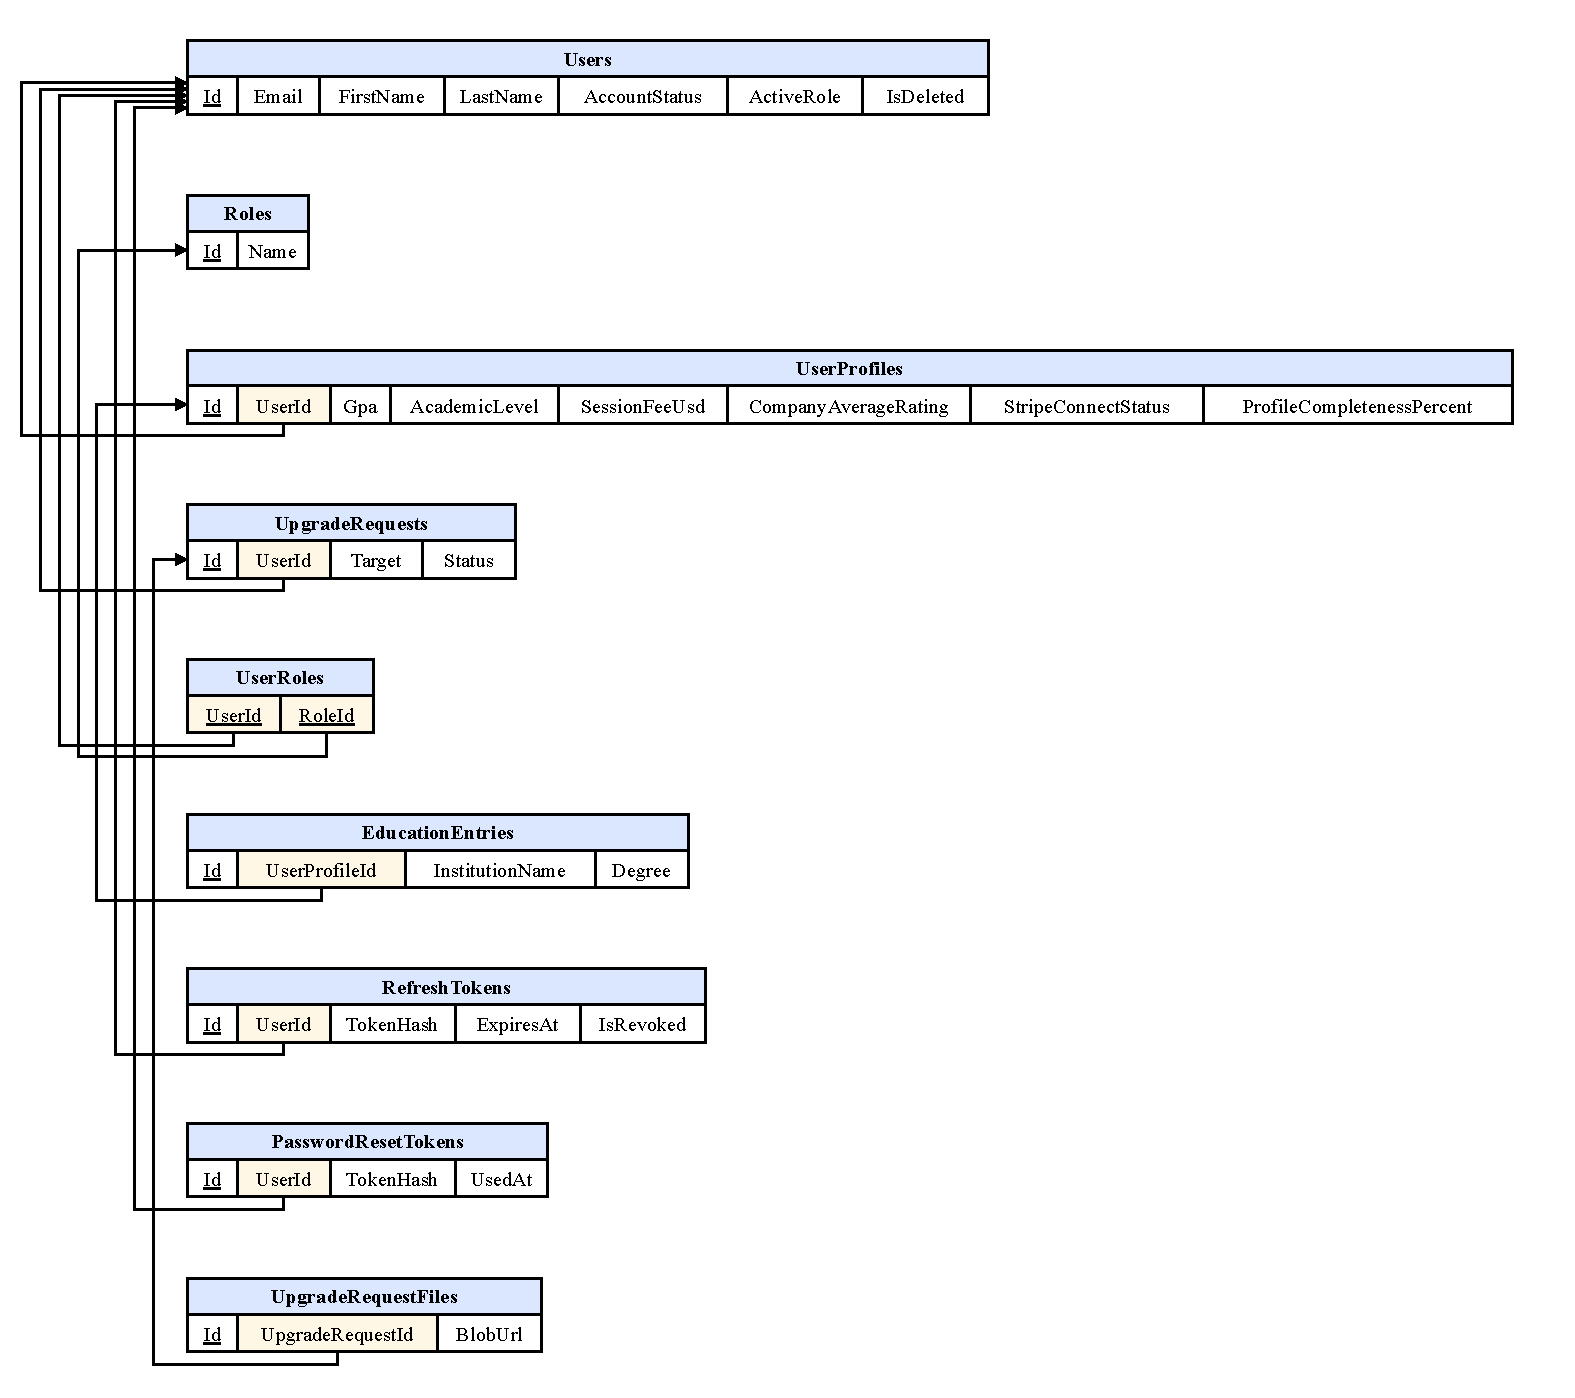
\includegraphics[width=\linewidth,height=0.82\textheight,keepaspectratio]{RelMap_Identity_Profile.pdf}
\caption{Relational mapping --- Identity, Access \& Profile. The
\texttt{Users}/\texttt{UserProfiles} pair shows the single-table specialization
(Step~8) plus the 1:1 link (Step~3); \texttt{UserRoles} is the M:N junction
(Step~5); \texttt{Education\_Entries} is the cascading weak entity (Step~2).}
\label{fig:identity}
\end{figure}

\subsection{Scholarships, Applications \& Documents}

Here \texttt{Scholarships}$\rightarrow$\texttt{Applications} is the central 1:N
(Step~4), \texttt{Scholarship\_Children} and \texttt{Application\_Children} are
weak EAV entities (Step~2), \texttt{SavedScholarships} is the uniqueness-only
M:N bookmark (Step~5), \texttt{CompanyReviewRequests} is the n-ary relationship
(Step~7), and \texttt{CompanyReviews} is the 1:1 review (Step~3).

\begin{figure}[H]\centering
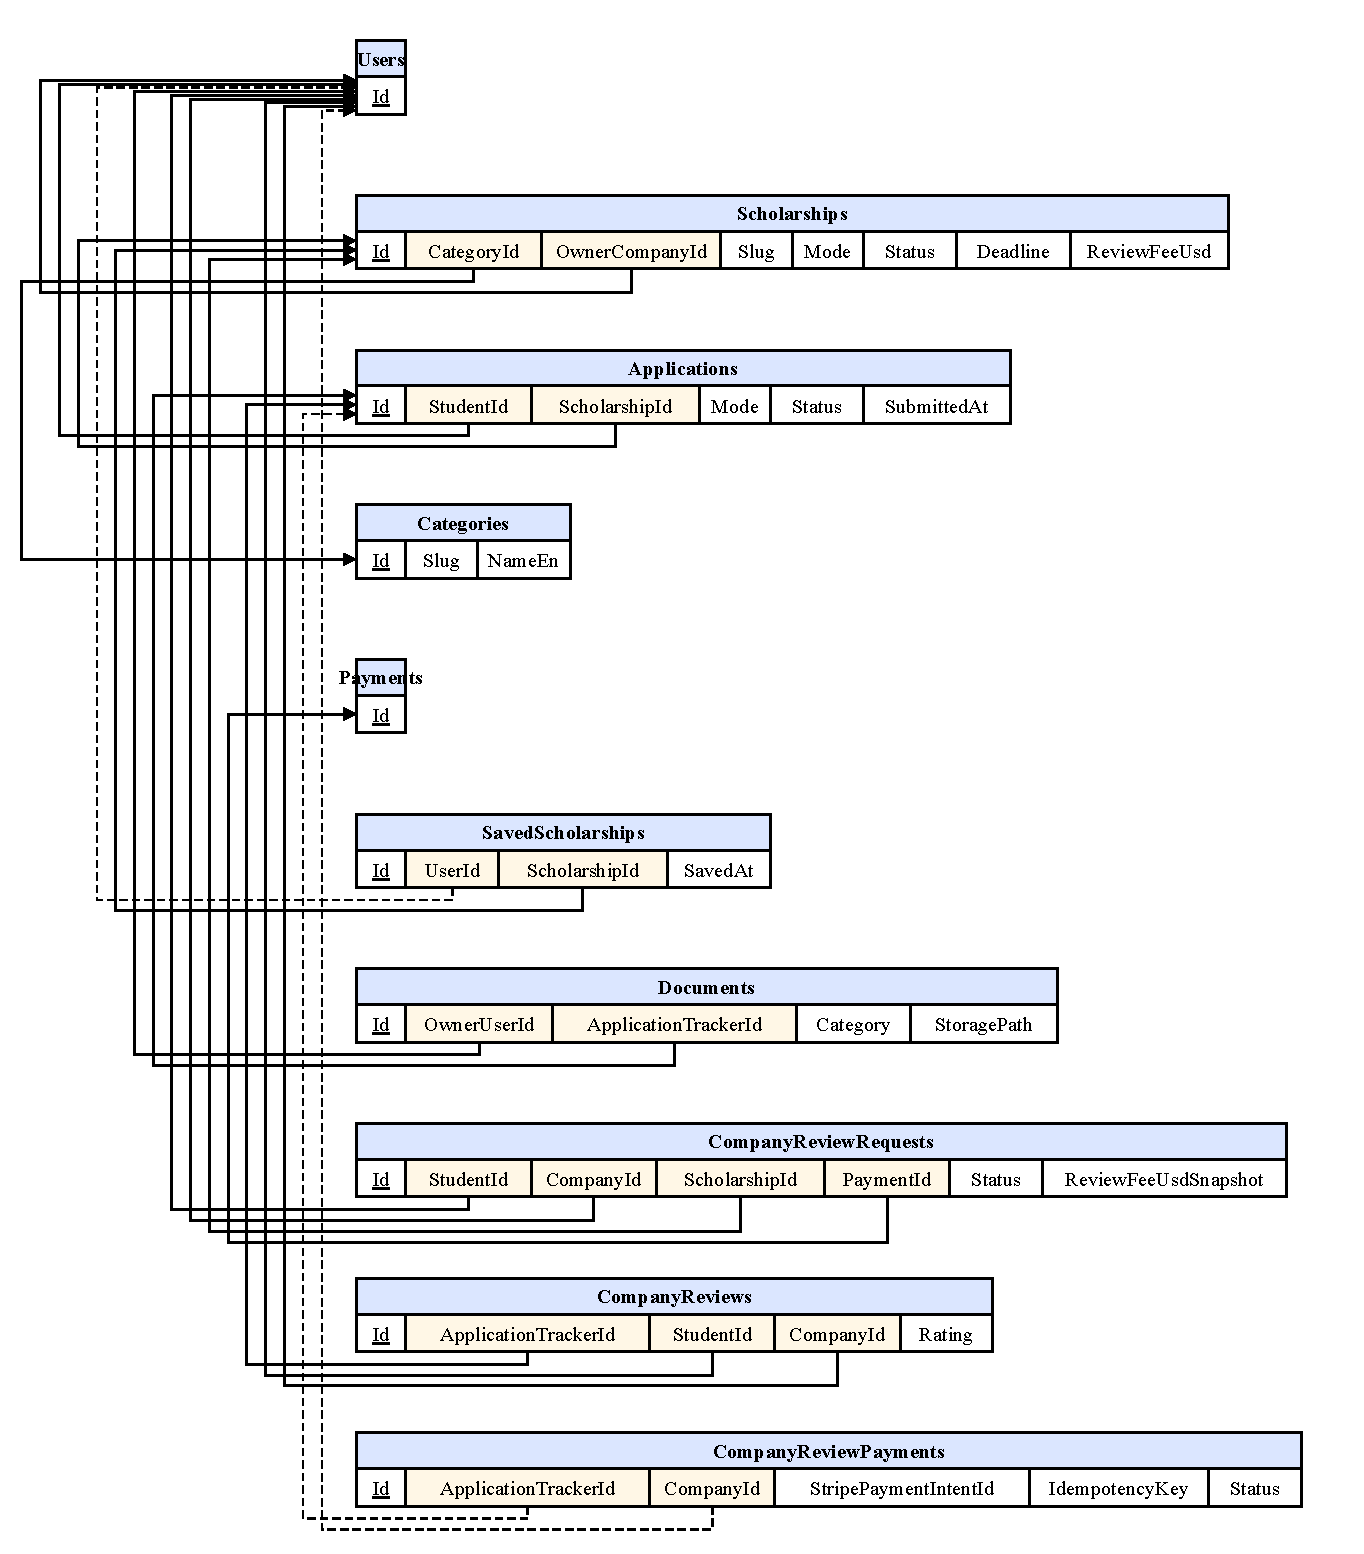
\includegraphics[width=\linewidth,height=0.82\textheight,keepaspectratio]{RelMap_Scholarships_Applications.pdf}
\caption{Relational mapping --- Scholarships, Applications \& Documents,
showing the n-ary \texttt{CompanyReviewRequests} relation and the
filtered-unique business rules.}
\label{fig:scholarships}
\end{figure}

\subsection{Consultant Booking, Payments \& Ratings}

This area contains \texttt{Availabilities}$\rightarrow$\texttt{Bookings} (1:N),
the \texttt{Bookings}--\texttt{ConsultantReviews} 1:1 (Step~3), the
financial-settlement relations (\texttt{Payments}, \texttt{Payouts}), and the
session-recording trail. It is the strongest illustration of two policies:
\emph{all} FKs into \texttt{Users} are \textbf{Restrict} (a booking references
\texttt{Users} twice --- student and consultant), and money for settlement is
stored as integer cents.

\begin{figure}[H]\centering

\includegraphics[width=\linewidth,height=0.82\textheight,keepaspectratio]{RelMap_Booking_Payments_Ratings.pdf}
\caption{Relational mapping --- Booking, Payments \& Ratings. \texttt{Payments}
and \texttt{Payouts} carry \emph{no} database foreign keys by design (loose
references); the booking's \texttt{(ConsultantId, ScheduledStartAt)}
filtered-unique index prevents double-booking.}
\label{fig:booking}
\end{figure}

\subsection{Community \& Chat}

The forum demonstrates a self-referencing 1:N (\texttt{ForumPosts} reply tree),
the \texttt{ForumPostTags} M:N junction (Step~5), and several cascading child
relations (votes, flags, bookmarks, attachments). The chat side
(\texttt{Conversations}, \texttt{Messages}, \texttt{UserBlocks}) leans heavily on
loose references to keep messaging decoupled from the user principal.

\begin{figure}[H]\centering

\includegraphics[width=\linewidth,height=0.82\textheight,keepaspectratio]{RelMap_Community_Chat.pdf}
\caption{Relational mapping --- Community \& Chat. \texttt{ForumPostTags} is the
true M:N junction; the \emph{user} leg of votes/flags/bookmarks and the chat
participant/sender legs are loose references.}
\label{fig:community}
\end{figure}

\subsection{Resources Hub \& Notifications}

\texttt{Resources}$\rightarrow$\texttt{ResourceChapters} is a cascading 1:N with
\texttt{ResourceChapters} as a weak entity (Step~2); progress and bookmark
tables hang off \texttt{Resources} with cascade, while their \texttt{UserId}
legs are loose. Notifications and notification preferences are fully
loose-referenced.

\begin{figure}[H]\centering

\includegraphics[width=\linewidth,height=0.82\textheight,keepaspectratio]{RelMap_Resources_Notifications.pdf}
\caption{Relational mapping --- Resources Hub \& Notifications, showing the
cascading chapter/progress children and the loose-referenced notification
tables.}
\label{fig:resources}
\end{figure}

\subsection{AI, Knowledge Base \& Platform}

The cross-cutting area holds \texttt{AiInteractions} with its 1:1
\texttt{AiRedactionAuditSamples} (Step~3), the
\texttt{RecommendationClickEvents} fact table, the
\texttt{KnowledgeDocuments} vector store, and the platform tables
(\texttt{PlatformSettings}, \texttt{AuditLogs}, \texttt{UserDataRequests},
\texttt{UserRiskFlags}). Most of these use loose references because they are
high-volume, audit, or analytics relations.

\begin{figure}[H]\centering

\includegraphics[width=\linewidth,height=0.82\textheight,keepaspectratio]{RelMap_AI_Platform.pdf}
\caption{Relational mapping --- AI, Knowledge Base \& Platform. \texttt{AuditLogs}
and \texttt{KnowledgeDocuments} use polymorphic soft references; \texttt{UserRiskFlags}
is a 1:1 analytics-fed relation.}
\label{fig:ai}
\end{figure}

\section{Referential-integrity strategy}
\label{sec:refint}

Foreign-key delete rules are not an afterthought; they encode how the data model
behaves under deletion and anonymization. ScholarPath uses four strategies,
summarized in Table~\ref{tab:refint}.

\begin{table}[H]\centering
\caption{Delete-rule strategy across the schema.}
\label{tab:refint}
\small
\begin{longtable}{@{}>{\raggedright\arraybackslash}p{2.2cm}>{\raggedright\arraybackslash}p{6.2cm}>{\raggedright\arraybackslash}p{6.0cm}@{}}
\toprule
\textbf{Rule} & \textbf{Used for} & \textbf{Why} \\
\midrule
\endhead
\textbf{Cascade} &
Education($\rightarrow$profile); upgrade files/links($\rightarrow$request);
scholarship-children \& saved-scholarships($\rightarrow$scholarship);
application-children($\rightarrow$application); forum
attachments/votes/flags/bookmarks/post-tags($\rightarrow$post/tag);
messages($\rightarrow$conversation); resource
chapters/bookmarks/progress/progress-children($\rightarrow$resource). &
The child has no meaning without its parent (existence dependency). \\
\addlinespace
\textbf{Restrict} &
\emph{Every} FK into \texttt{Users} (profile, refresh/reset tokens,
upgrade-request, user-risk-flag, applications, documents, bookings, all reviews,
recordings, recommendation clicks, redaction samples). &
Protect history; and avoid SQL~Server's \emph{multiple cascade paths} error
(1785) --- a row may reference \texttt{Users} two or three times. \\
\addlinespace
\textbf{SetNull} &
scholarship$\rightarrow$category, scholarship$\rightarrow$owner-company,
document$\rightarrow$application, booking$\rightarrow$availability/payment,
request$\rightarrow$payment, post$\rightarrow$category. &
Keep the row but orphan an \emph{optional} link. \\
\addlinespace
\textbf{none (loose)} &
payments, payouts, notifications, the \emph{user} leg of
votes/flags/bookmarks, chat participants/sender, audit actor + target, AI
\texttt{UserId}, knowledge \texttt{SourceId}, settings/requests/stories user. &
Decouple high-volume / audit / analytics rows from the principal so deletes and
anonymization never cascade-break. \\
\bottomrule
\end{longtable}
\end{table}

The single most important defense point: \textbf{no foreign key cascades out of
\texttt{Users}}. Every \texttt{\dots\_Users\_\dots} foreign key --- including the
1:1 keys on \texttt{UserProfiles} and \texttt{UserRiskFlags} and the
\texttt{UserRoles} join --- is \texttt{ON DELETE NO ACTION} (Restrict).
Cascading deletes originate only from the \emph{aggregate roots} listed in the
Cascade row (Scholarship, Application, ForumPost, Resource, Conversation,
UpgradeRequest, and UserProfile$\rightarrow$Education). This protects audit and
financial history and side-steps SQL~Server's multiple-cascade-paths
restriction, since several relations reference \texttt{Users} more than once.

\section{Accuracy: model versus live database}
\label{sec:accuracy}

A graduation defense rewards precision about what the \emph{deployed} database
actually enforces, as opposed to what the conceptual model implies. Three points
were verified directly against the live Azure SQL dump and deserve emphasis,
because each is a place where the database does \emph{not} match the naive
reading of the model.

\begin{enumerate}[leftmargin=1.6em]
  \item \textbf{The single-active-application rule (FR-057) is enforced in
        application code only.} There is \emph{no} DB filtered-unique index on
        \texttt{Applications} in production. The historical
        \texttt{UX\_Applications\_Student\_Scholarship\_Active} index was dropped
        when \texttt{ScholarshipId} became nullable (migration
        \texttt{20260521163702}, to allow external-tracker applications with no
        scholarship) and was never recreated. So ``one active application per
        (student, scholarship)'' is a guarantee made by the service layer, not
        the schema.

  \item \textbf{By contrast, \texttt{CompanyReviewRequests} and
        \texttt{Bookings} \emph{do} have DB-enforced filtered-unique indexes.}
        \texttt{CompanyReviewRequests} keeps
        \texttt{(StudentId, ScholarshipId)} unique \texttt{WHERE Status IN
        ('Draft','Submitted','Pending','UnderReview')}, and \texttt{Bookings}
        keeps \texttt{(ConsultantId, ScheduledStartAt)} unique \texttt{WHERE
        Status IN ('Requested','Confirmed')}. These business rules are
        guaranteed by the database, not merely by code. The contrast with
        point~(1) is the kind of detail a committee will probe, so it is stated
        plainly.

  \item \textbf{Money is stored two different ways, on purpose.}
        Settlement-grade money (the \texttt{Payments} and \texttt{Payouts}
        relations: \texttt{AmountCents}, \texttt{PayeeAmountCents},
        \texttt{RefundedAmountCents}, etc.) is stored as \texttt{bigint}
        \emph{integer cents}, the standard way to avoid floating-point and
        rounding errors in financial settlement. Display-grade money (prices and
        fees: \texttt{PriceUsd}, \texttt{SessionFeeUsd}, \texttt{ReviewFeeUsd},
        \texttt{FundingAmountUsd}) is stored as \texttt{decimal(p,2)}. The split
        is deliberate: cents for arithmetic that must reconcile to the last unit,
        decimal for catalog values that are only ever displayed or compared.
\end{enumerate}

A handful of relations are also documented as \emph{schema-only / planned} or
\emph{legacy / dead} (e.g.\ \texttt{ForumPostAttachments},
\texttt{SuccessStories}, and \texttt{CompanyReviewPayments}); they exist in the
schema for completeness but have no live write path. Documenting them as such ---
rather than pretending they are active --- is part of keeping the mapping honest.

If a reviewer wants the authoritative DDL, the project can regenerate it straight
from the migrations:

\begin{lstlisting}[language=bash]
cd server
dotnet ef migrations script \
  --project src/ScholarPath.Infrastructure \
  --startup-project src/ScholarPath.API \
  > ../docs/diagrams/schema.sql
\end{lstlisting}

\section{Closing}

Applying Elmasri \& Navathe's seven/nine-step algorithm to the Part~2 EERD
yields the ScholarPath relational schema: \textbf{62 tables deployed} to Azure
SQL, every one traceable back to a specific conceptual construct via
Table~\ref{tab:algo}. Strong entities became relations, weak entities became
cascading child relations, 1:1 links became unique foreign keys, M:N
relationships became junction tables, the user hierarchy became a single
discriminated table, and the n-ary review workflow became a four-foreign-key
relation --- with deliberate, documented deviations (JSON multivalued columns,
loose references) where the deployed schema favors pragmatism over textbook
purity.

This completes the relational view. The \emph{object-oriented} view --- how
these relations map back to C\# entity classes, aggregates, and navigation
properties --- is the subject of \emph{ScholarPath --- Class Diagrams}
(Part~4).

\end{document}
